\section{Analizowane ziarna rud miedzi} \label{sec:grains}
Zestaw analizowanych ziaren pochodzi z~projektu \textsc{sysmel} (\emph{System
sterowania procesem mielenia w~układzie z~młynem elektromagnetycznym})
\footnote{Pełen tytuł projektu naukowego: \emph{Układ mielenia surowców
mineralnych w~młynie elektromagnetycznym wraz z~systemem sterowania jego
pracą, zapewniający wysoką efektywność technologiczną i~niską energochłonność
w~zastosowaniach mikro i~makro-przemysłowych.}},
którego współtwórcami są naukowcy z~Politechniki Śląskiej.
Uzyskane próbki powstały w~procesie mielenia rud miedzi w~młynie
elektromagnetycznym.
Poszczególne klasy ziaren różnią się granulacją i~parametrami procesu
ich mielenia.
Spośród próbek, pochodzących z~projektu \textsc{sysmel}, wybrano cztery
typy ziaren, które będą przedmiotem zadania klasyfikacji.
Zdjęcia rozpatrywanych materiałów przedstawiono na rysunku \ref{fig:grains}.
\begin{figure}[htb]
    \centering
	\begin{subfigure}[t]{0.35\textwidth}
		\centering
		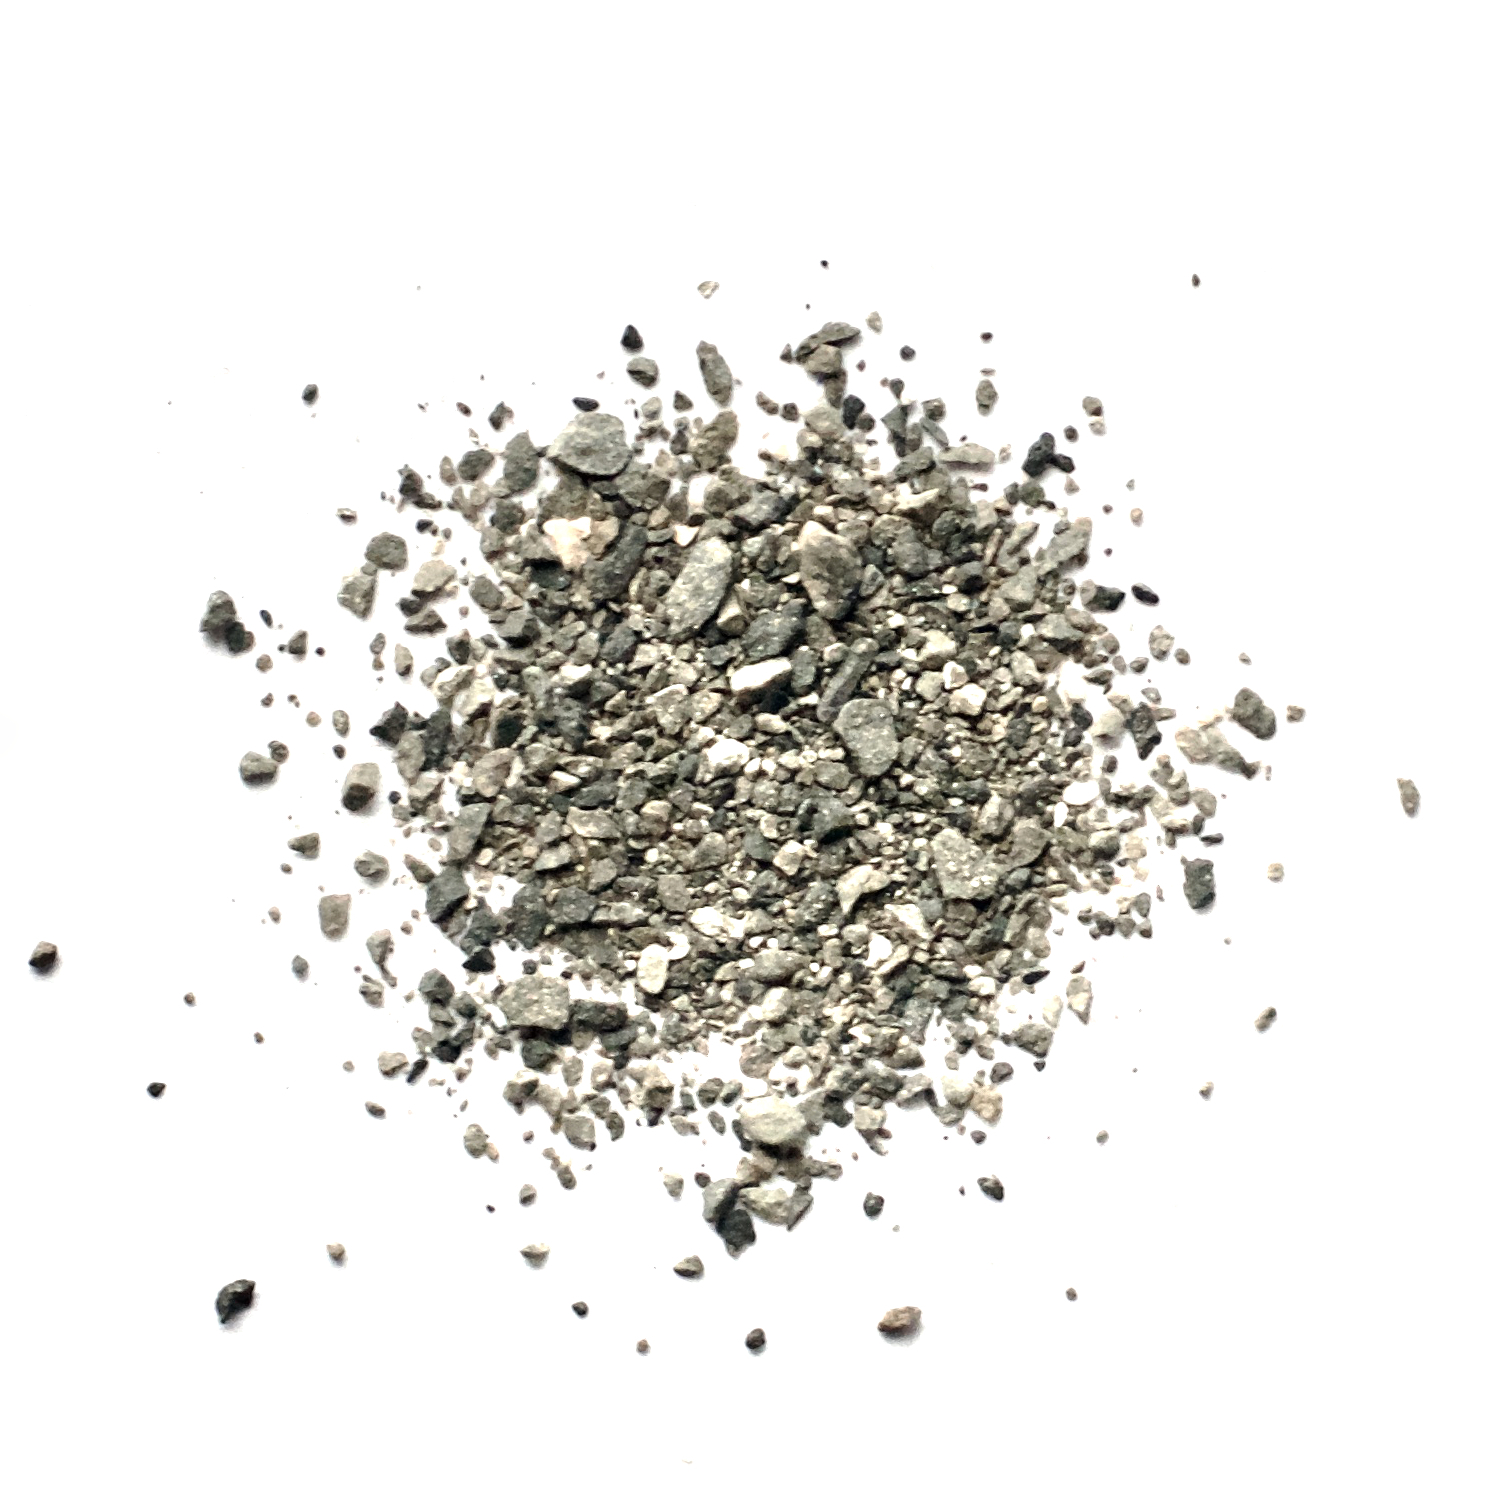
\includegraphics[width=\textwidth]{E5R}
		\caption{Ziarna rudy miedzi klasy E5R}
	\end{subfigure}
	\quad\quad
	\begin{subfigure}[t]{0.35\textwidth}
		\centering
		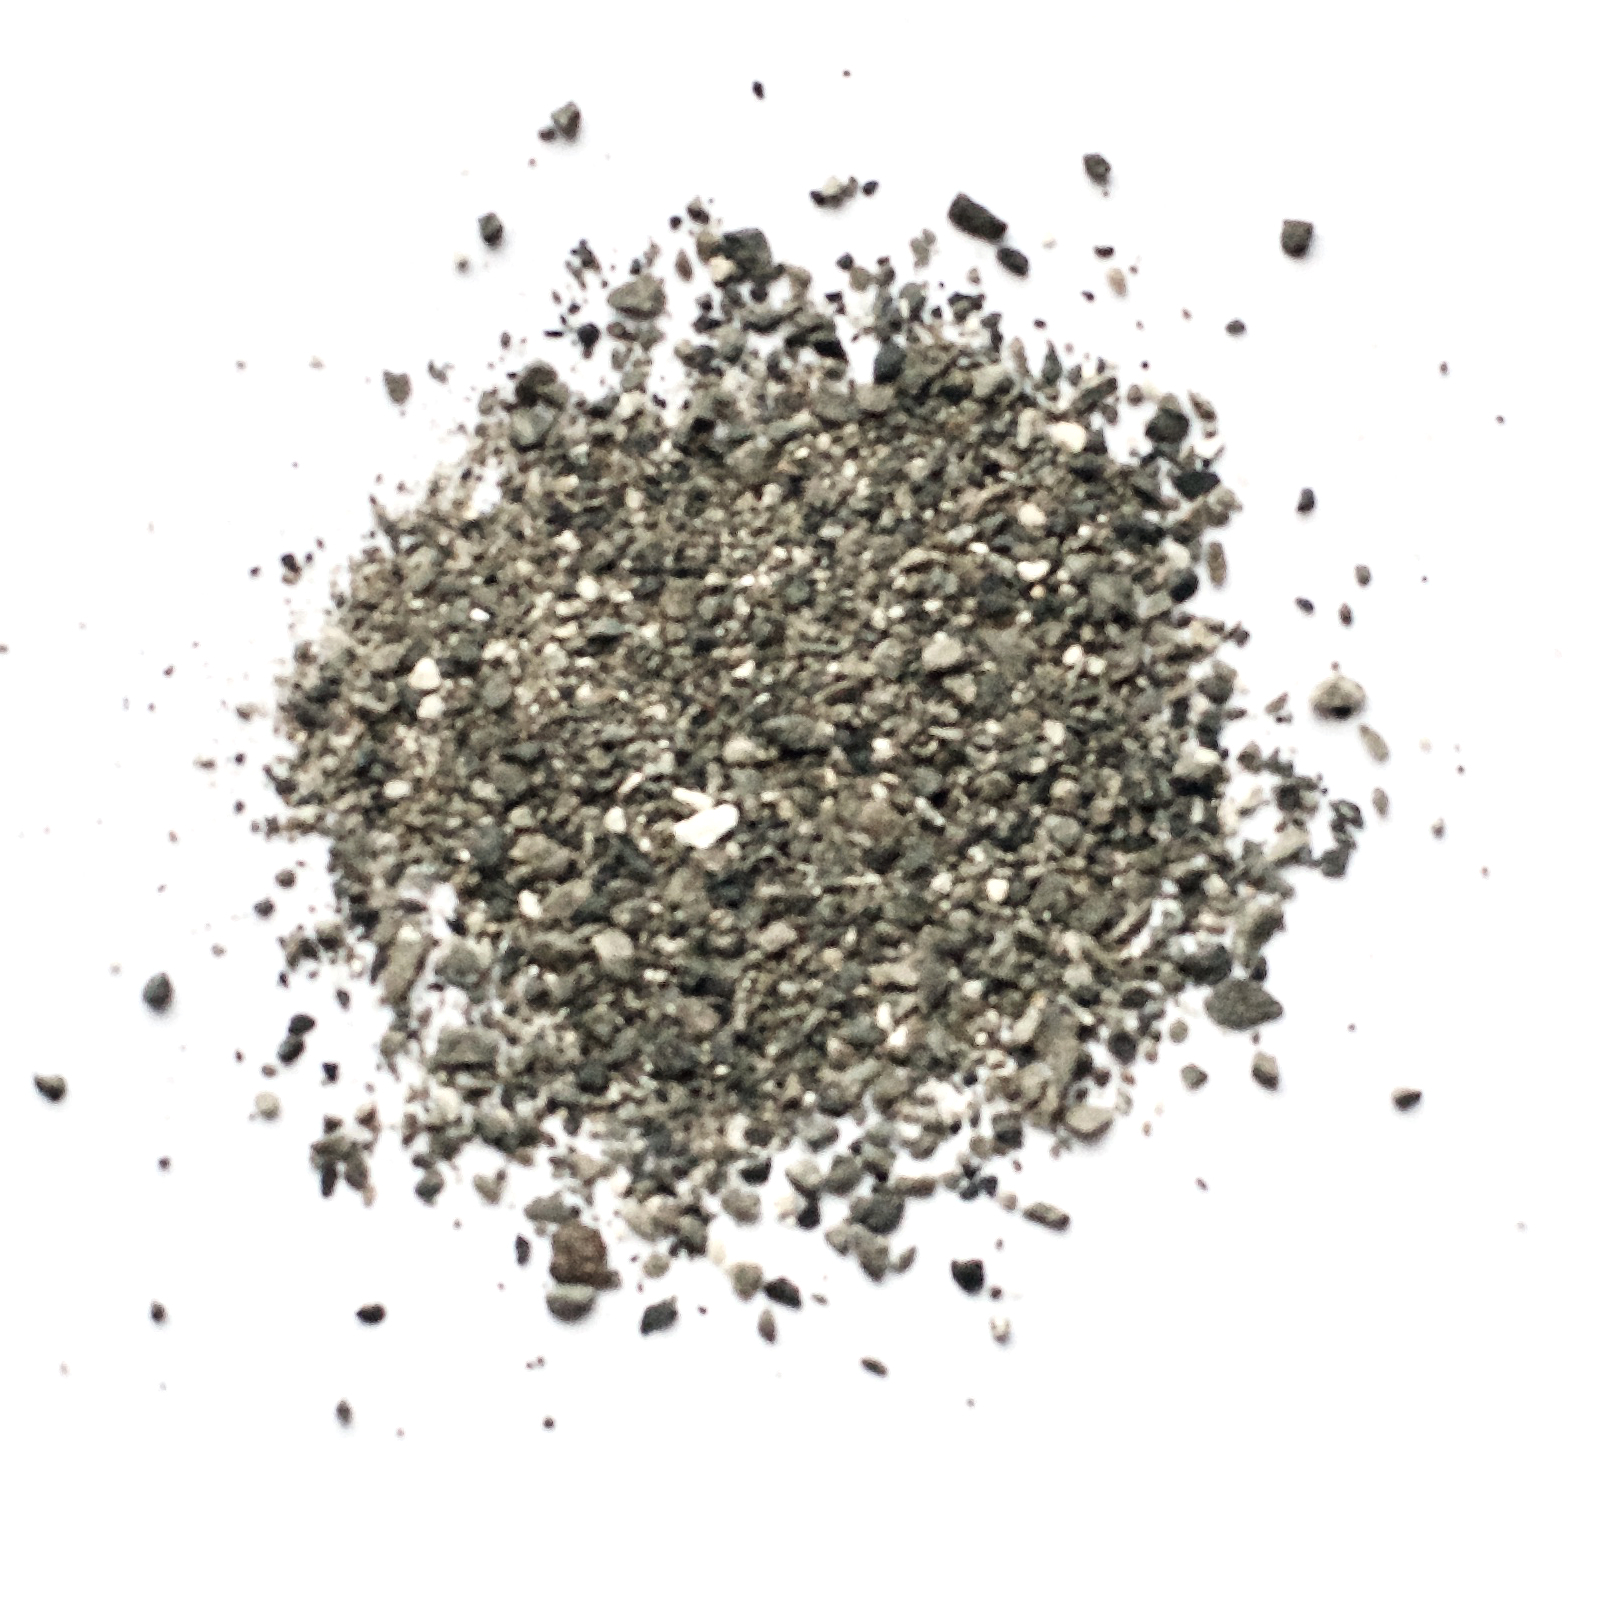
\includegraphics[width=\textwidth]{E6R}
		\caption{Ziarna rudy miedzi klasy E6R}
	\end{subfigure}
	\vskip\baselineskip
	\begin{subfigure}[t]{0.35\textwidth}
		\centering
		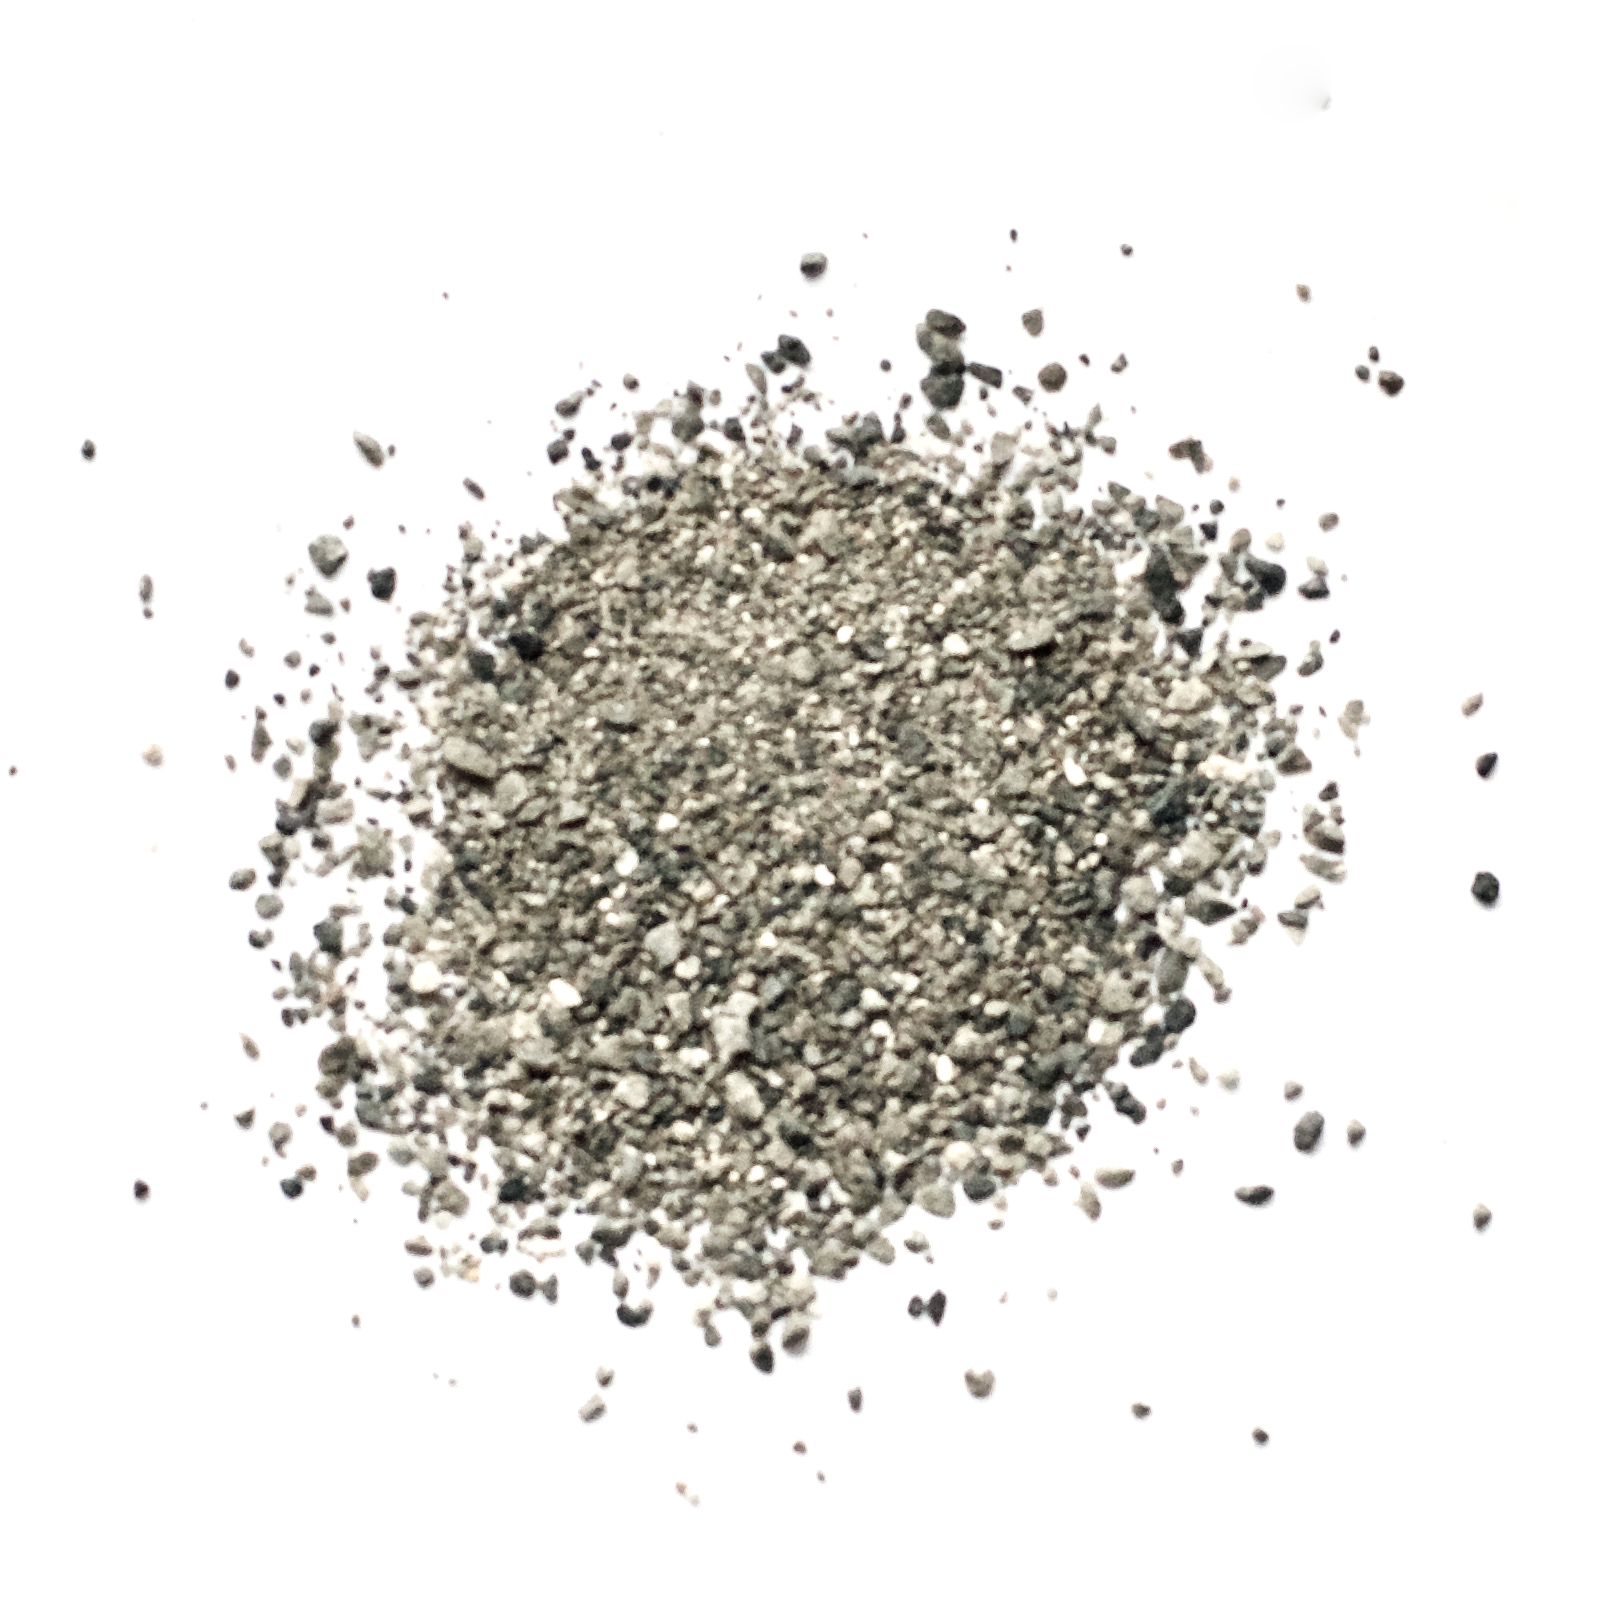
\includegraphics[width=\textwidth]{E11R}
		\caption{Ziarna rudy miedzi klasy E11R}
	\end{subfigure}
	\quad\quad
	\begin{subfigure}[t]{0.35\textwidth}
		\centering
		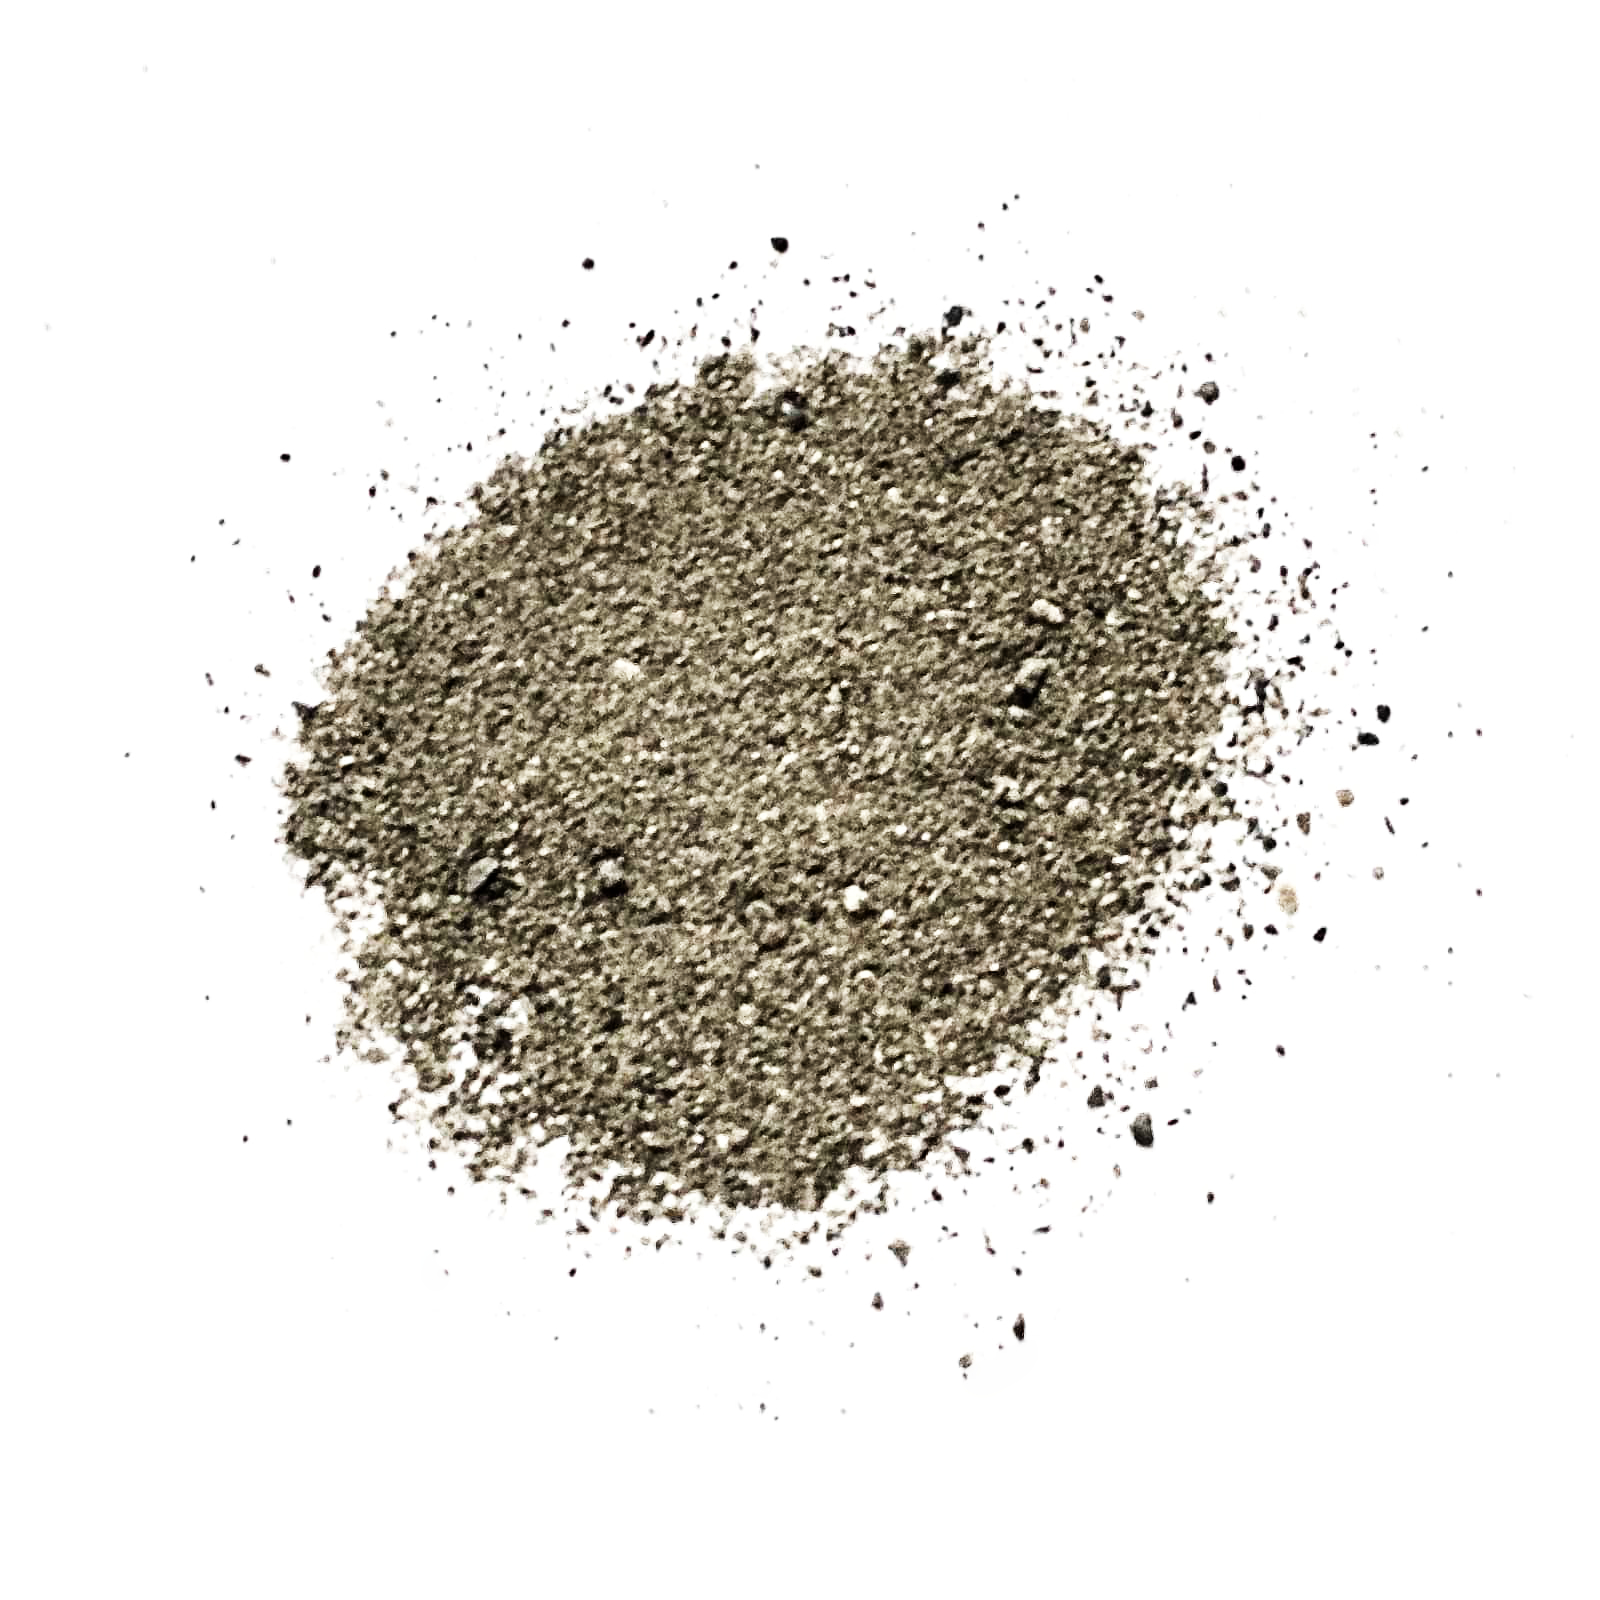
\includegraphics[width=\textwidth]{E16R}
		\caption{Ziarna rudy miedzi klasy E16R}
	\end{subfigure}
	\caption{Próbki rozpatrywanych ziaren rud miedzi}
	\label{fig:grains}
\end{figure}

\section{Metody pomiarów termowizyjnych}
\label{sec:thermovision}
Pomiary termowizyjne (nazywane także \emph{termografią}) polegają na
rejestracji promieniowania cieplnego obiektów w~celu ustalenia ich
temperatury.
Badania z~wykorzystaniem termowizji można podzielić na dwie grupy:
\emph{termowizję pasywną} oraz \emph{termowizję aktywną}.

Technika pasywna polega na rejestracji obrazów obiektów bez ingerencji w~ich
temperaturę w~czasie trwania pomiarów.
Można w~ten sposób obserwować przepływ ciepła w~urządzeniach technicznych,
procesach przemysłowych oraz biologicznych.
W~rozważanym w~pracy przypadku technika ta nie ma jednak zastosowania.
W~warunkach pokojowych badany materiał ma w~całej swojej objętości podobną
temperaturę, co skutkuje obrazem równomiernego szumu w~rejestrowanym obrazie.

Bardziej zaawansowaną techniką są pomiary z~wykorzystaniem termowizji
aktywnej.
W tym trybie pomiarów badane obiekty ogrzewa się w~powtarzalnych warunkach, 
a~następnie rejestruje proces ich stygnięcia.
Podczas dostarczania ciepła do obiektu oraz jego oddawania na obrazach
termowizyjnych można zaobserwować strukturę badanego obiektu.
Przedmioty o~niejednorodnej i~złożonej budowie nagrzewają się oraz stygną
nierównomiernie, co jest rejestrowane przez kamery termowizyjne.
W~ten sposób można dostrzec cechy obiektu niewidoczne gołym okiem, takie
jak zmiany jego gęstości, składu oraz uszkodzenia struktury.
Termowizję aktywną stosuje się szeroko w~badaniach naukowych oraz przemyśle.
Przykładowe aplikacje tej techniki to detekcja defektów w~produktach
przemysłowych oraz wykrywanie części konstrukcji podatnych na zużycie.
Termowizja aktywna ma charakter niedestruktywny oraz bezkontaktowy,
co stanowi jej zalety w~analizie materiałowej \cite{ciampa_thermography}.
Technika ta wymaga jednak etapowego procesu pomiarowego, potrzebne jest 
przygotowanie instalacji grzewczej, a~nagrzewanie i~stygnięcie materiału
może być czasochłonne.
Przebieg zmian temperatury najlepiej rejestrować na materiałach wideo,
aby zmaksymalizować ilość danych zgromadzonych w~trakcie eksperymentu.

\section{Kamera termowizyjna FLIR A320}
\label{sec:camera}
Przedmiotem projektu jest analiza obrazów pochodzących z~przemysłowej
kamery termowizyjnej FLIR A320.
Firma FLIR zajmuje się produkcją wysokiej jakości kamer i~detektorów do celów
profesjonalnych i~przemysłowych.
Używany aparat łączy wysoką jakość pomiaru z~nowoczesnymi funkcjami
integracji z~oprogramowaniem komputerowym.
Urządzenie komunikuje się z~komputerem za pomocą sieci internetowej,
pozwalając na kontrolę z~poziomu aplikacji oraz bibliotek
programistycznych.
Dodatkowo kamera posiada możliwość planowania automatycznych pomiarów
i~alarmów, oferuje także funkcje analityczne oraz wbudowany serwer
internetowy \cite{flir_a32x_manual}.

\subsection{Opis sprzętowy wykorzystywanej kamery}
Kamera ma postać podłużnego korpusu, do którego swobodnie można podłączać
obiektywy.
Na rysunku \ref{fig:camera}~przedstawiono zdjęcie wykorzystywanego urządzenia.
\begin{figure}[htb]
    \centering
    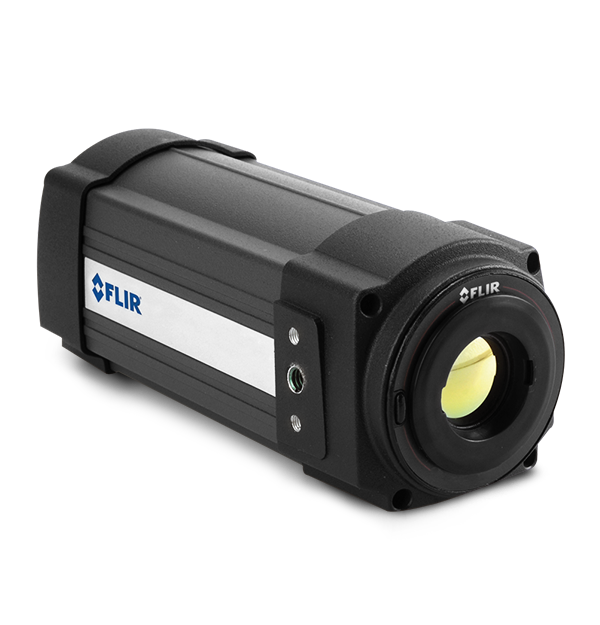
\includegraphics[width=0.5\textwidth]{flir_a320}
    \caption{Kamera termowizyjna FLIR A320 \cite{flir_camera_specs}}
    \label{fig:camera}
\end{figure}
Egzemplarz kamery znajdujący się w~laboratorium termowizji Politechniki
Śląskiej został wyposażony w~obiektyw, pozwalający oglądać ziarna rud miedzi
w~powiększeniu.
Kamera cechuje się następującymi parametrami \cite{flir_camera_specs}:
\begin{itemize}
	\item typ detektora: niechłodzony mikrobolometr
	\item rozdzielczość: 320 na 240 pikseli,
	\item częstotliwość odświeżania: \SI{9}{\hertz} do \SI{30}{\hertz}
	\item szerokość otworu: \textit{f}\num{1,3},
	\item autofokus z wbudowanym silnikiem,
	\item zakres pomiarowy temperatur: 
		\begin{enumerate}
			\item od \SI{-15}{\celsius} do \SI{+50}{\celsius},
			\item od \SI{0}{\celsius} do \SI{350}{\celsius},
		\end{enumerate}
	\item dokładność: \num{\pm2}\si{\celsius} lub \num{\pm2}\% odczytu,
	\item zakres wykrywanego widma promieniowania: \SI{7,5}{\micro\meter}
          do \SI{13}{\micro\meter}.
\end{itemize}

Kamera wykrywa temperaturę przez detektor zwany \emph{bolometrem},
który mierzy energię niesioną przez fale elektromagnetyczne w~spektrum
podczerwieni.
Kiedy fala pada na detektor aparatu, temperatura komórek matrycy rośnie
i~zwiększa się ich rezystancja elektryczna.
Wartości rezystancji są mierzone, a~na ich podstawie określana jest
temperatura \cite{vanhoof_infrared}.

Zakres temperatur kamery jest odpowiedni do przeprowadzenia eksperymentów
z~pomiarami ziaren rud miedzi metodą termowizji aktywnej.
Próbki planuje się podgrzewać do temperatury maksymalnie około
\SI{80}{\celsius},~wartość ta mieści się w~zakresie pracy urządzenia.
Dokładność kamery jest zadowalająca, próbne materiały nagraniowe
wskazały, że na zdjęciach widocznych jest wiele szczegółów i~detali
badanego materiału.
Przy klasyfikacji obrazów i~wzorców stygnięcia próbek jest to 
bardziej istotne niż liczbowa dokładność pomiarowa przyrządu.

W~porównaniu ze zwykłymi, współczesnymi aparatami, rozdzielczość kamery
termowizyjnej może wydawać się mała.
Należy sobie jednak uzmysłowić, że w~standardowych aparatach piksele mają
rozkład Bayera, a~wartości składowych koloru są interpolowane.
W~kamerze termowizyjnej każda komórka matrycy dokonuje pełnego pomiaru
wartości temperatury.
Z~tego powodu bezpośrednie porównanie rozdzielczości używanego
przyrządu z~popularnymi aparatami może być mylące.
Oczywiście większa rozdzielczość kamery byłaby pożądana, jednak jej obecne
możliwości pozwalają na szczegółowe pomiary i~obserwację wielu detali ziaren
rud miedzi.

\subsection{Obiektyw kamery}
\label{subsec:lens}
Kamerę wyposażono w~obiektyw zbliżeniowy FLIR~T197415, pozwalający obserwować
ziarna rud miedzy.
Jest to sprzęt zaprojektowany przez producentów używanej kamery i~dedykowany
pracy z~urządzeniami termowizyjnymi.
Przyrząd przedstawiono na rysunku \ref{fig:lens}.
\begin{figure}[htb]
    \centering
    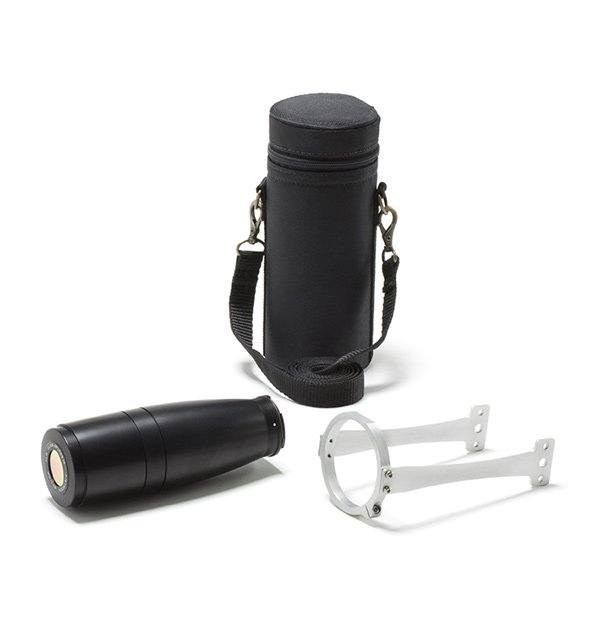
\includegraphics[width=0.5\textwidth]{flir_lens}
    \caption{Obiektyw FLIR T197415 \cite{flir_lens_specs}}
    \label{fig:lens}
\end{figure}
Wybrany obiektyw jest przygotowany z~myślą o~obserwacji drobnych detali
powierzchni w~dużym zbliżeniu.
Używany model ma następujące parametry \cite{flir_lens_specs}:
\begin{itemize}
	\item ogniskowa: \SI{18,2}{\milli\meter},
	\item powiększenie: \num{1x1},
	\item pole widzenia: \SI{8}{\milli\meter} na \SI{6}{\milli\meter},
	\item odległość od płaszczyzny ostrzenia: \SI{20}{\milli\meter},
	\item głębia ostrości: \SI{0,3}{\milli\meter},
	\item przysłona: bez regulacji, równa otworowi systemu montażu kamery,
	\item budowa: trzy soczewki asferyczne.
\end{itemize}

Zgodnie ze specyfikacją producenta obiektyw ma powiększenie \num{1x1},~co
może wydawać się niedużą wartością.
Należy mieć jednak świadomość, że zwykłe obiektywy zmniejszają obraz
padający na matrycę.
Powszechnie  jako granicę makrofotografii przyjmuje się
powiększenie \num{1x1}.~
W~obserwacji ziaren i~detali powierzchni nie jest jednak istotne powiększenie,
ale to że używany obiektyw jest \emph{zbliżeniowy}.
Oznacza to, że ma on bardzo małą odległość ostrzenia, czyli można go przysunąć
blisko obserwowanej powierzchni.
Obiektyw zbliżeniowy pozwala na obserwację z~dystansu
\SI{20}{\milli\meter},~typowe obiektywy ostrzą z~odległości parudziesięciu
centymetrów do ponad metra.
Dzięki temu obiektyw zbliżeniowy pozwala na obserwację bardzo drobnych
detali powierzchni.

\subsection{Oprogramowanie do obsługi kamery}
\label{subsec:camera_soft}
Jedną z~najważniejszych cech kamery jest łatwość integracji
z~oprogramowaniem komputerowym.
Kamerę można obsługiwać za pomocą programu FLIR Tools\footnote{Strona produktu
programu FLIR Tools: \url{https://www.flir.com/products/flir-tools/}}.
Pozwala on na podgląd obrazu oraz wykonywanie zdjęć termowizyjnych.
Producent dostarcza również bibliotekę LabVIEW pozwalającą na zaawansowaną
pracę z~kamerą.
Do obsługi stanowiska został napisany program używający tych bibliotek,
który pozwala na nagrywanie materiałów wideo przy pomocy kamery.
Nagrania mają własnościowy format firmy FLIR, można je odtwarzać w~programie
FLIR Tools.
Program pozwala także na eksport stopklatek z~nagrania w~postaci plików JPEG.
Przy obsłudze narzędzia ważne jest ustawianie zakresu temperatur na obrazie.
Wybrany zakres określa w~jaki sposób wartości temperatury są mapowane na
kolory na zdjęciu, zawarte w~tablicy LUT.
Program oferuje tablice w~skali szarości, takie zostały użyte w~projekcie,
możliwy jest także wybór tablic w~postaci kolorowych gradientów.
Wybór zakresu wpływa na wygląd wyświetlanego obrazu oraz eksportowanych
stopklatek.
Jego nieodpowiedni dobór może skutkować zbyt ciemnym, jasnym, lub mało
kontrastowym obrazem.
Aby zapewnić najlepsze wykorzystanie nagrań z~kamery oraz powtarzalny
charakter eksportu stopklatek korzystano z~opcji automatycznego doboru
zakresu temperatur, jaki jest wbudowany w~program FLIR Tools.

\section{Narzędzia programistyczne}

\subsection{Język programowania Python}
Założenia projektu wymagają użycia języka programowania pozwalającego
na zaawansowaną obróbkę obrazu oraz wydajne budowanie sieci neuronowych.
W~obu tych dziedzinach wiodącym językiem jest Python, posiadający bogaty
zestaw bibliotek.
Język ten oferuje dużą wygodę programowania, co jest istotne przy pracy 
badawczej.
Jednocześnie Python jest zaopatrzony w~wydajną bibliotekę obliczeń
numerycznych NumPy.
Oferuje ona klasy macierzy numerycznych oraz bogaty zestaw operacji
matematycznych.
Macierze biblioteki NumPy są mniej elastyczne od zwykłych list języka Python,
jednak oferują dużo większą wydajność obliczeniową, między innymi dzięki
wsparciu obliczeń wektorowych na odpowiednich procesorach.
Wiele innych bibliotek języka wykorzystuje pakiet NumPy, na przykład przy
przetwarzaniu obrazów, co pozwala na wysoką wydajność obliczeń.
Połączenie wygody programowania z~zadowalającą wydajnością bibliotek
numerycznych, sprawia że Python jest dobrym wyborem do realizacji
założeń projektu.

\subsection{Biblioteka przetwarzania obrazu Scikit-image}
Język Python oferuje bogaty zestaw bibliotek przetwarzania obrazu.
Najbardziej popularną z~nich jest biblioteka OpenCV napisana w~języku
C\texttt{++}.
Zdecydowano się jednak na wybór mniej znanego pakietu Scikit-image.
Jest to biblioteka zorientowana na obliczenia naukowe i~badawcze
oraz napisana bezpośrednio z~myślą o~języku Python \cite{scikit-image}.
Scikit-image, w~porównaniu z OpenCV, oferuje bardziej spójny interfejs
programisty oraz lepiej wykorzystuje charakterystykę języka Python.
Dodatkowo wybrana biblioteka jest częścią zestawu Scikit, w~skład
którego wchodzi pakiet Scikit-learn służący do uczenia maszynowego.
Może on być przydatny przy tworzeniu sieci neuronowej, a~spójność bibliotek
z~pakietu Scikit jest niewątpliwie zaletą.
Wybrana biblioteka charakteryzuje się również dobrą dokumentacją
\cite{scikit_reference} oraz zestawem przykładów.

\subsection{Interfejs sieci neuronowych Keras}
\label{subsec:software_network}
Wybór bibliotek głębokiego uczenia w~języku Python jest bardzo szeroki.
Do najpopularniejszych pakietów należą: Keras, TensorFlow oraz PyTorch.
Zdecydowano się na wybór interfejsu biblioteki Keras.
Jest to pakiet nastawiony na elastyczność i~możliwość eksperymentowania,
oferuje wysokopoziomową, matematyczną warstwę abstrakcji opisu sieci
neuronowych \cite{chollet_keras}.
Moduł Keras oferuje także rozbudowaną dokumentację oraz zestaw poradników
\cite{keras_docs}.
Keras nie jest jednak pełnym rozwiązaniem, a~raczej abstrakcyjnym interfejsem.
Używanie go wymaga wyboru wewnętrznego silnika biblioteki.
Zdecydowano się na domyślną opcję użycia zaplecza pakietu TensorFlow.
W~standardowy sposób interfejsu Keras używa się po osobnym zainstalowaniu
jego modułów i~wskazaniu silnika sieci neuronowych.
Biblioteka TensorFlow udostępnia jednak wewnętrzny interfejs Keras,
co pozwala na zwiększenie wydajności obliczeniowej w~połączeniu dwóch
bibliotek.
Przy tworzeniu oprogramowania wzięto to pod uwagę i~użyto bardziej wydajnej
metody importowania interfejsu Keras.
